\documentclass[hyperref={pdfpagelabels=false}]{beamer}
\usepackage[ngerman]{babel}
\usepackage[utf8]{inputenc}
\usepackage{tikz}
\usepackage{listings}
\mode<presentation> { \usetheme{Montpellier} }
\lstset{language=Haskell, showstringspaces=false, basicstyle=\footnotesize}

\title{Text-basiertes Adventure-Game}
\author{Eva Braß, Felix Reihl}
\subtitle{Projekt für die Vorlesung Fortgeschrittene Funktionale Programmierung\\Wintersemester 1014/15}

\logo{\pgfputat{\pgfxy(-.5,8.05)}{\pgfbox[center,base]{
\includegraphics[width=1.1cm]{LMU_Siegel.pdf}}}}

\beamerdefaultoverlayspecification{<+->}
\begin{document}
% ---
\begin{frame} \titlepage
\end{frame} 
% ---
\begin{frame}
  \tableofcontents
\end{frame} 
% ---
\section{Das Spiel}
\begin{frame}
  \frametitle{Das Spielprinzip}
  \begin{itemize}
    \item Vorbild: Zork, Colossal Cave Adventure
    \item Per Texteingabe gibt der Spieler Anweisungen.
    \item Alle Geschehnisse und Beschreibungen werden als Text ausgegeben.
  \end{itemize}
\end{frame} 
% ---
\begin{frame}
  \frametitle{Spielablauf}
  \begin{figure}
    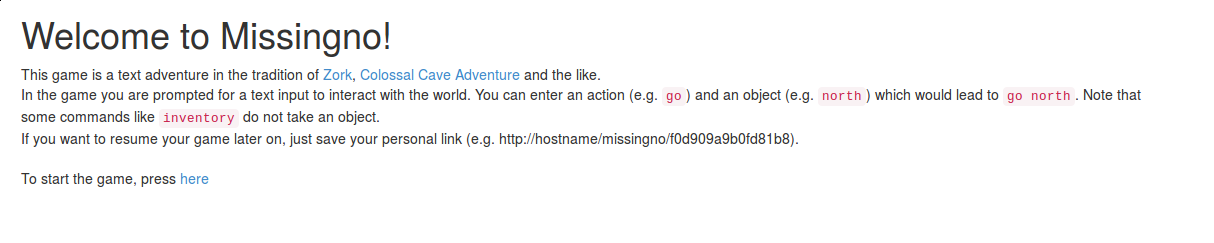
\includegraphics[scale=0.25]{screenshots/2015-03-25-103845_1214x243_scrot.png}
    \caption{Startseite}
  \end{figure}
  \begin{figure}
    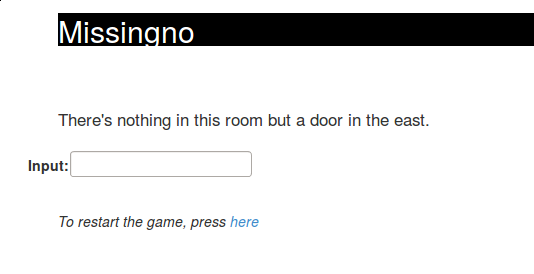
\includegraphics[scale=0.2]{screenshots/2015-03-25-104814_534x274_scrot.png}
    \caption{Erster Raum}
  \end{figure}
\end{frame}
% ---
\begin{frame}
  \begin{figure}
    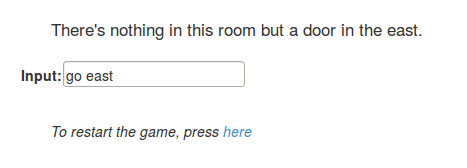
\includegraphics[scale=0.25]{screenshots/2015-03-25-104448_467x168_scrot.png}
    \caption{Aktion im ersten Raum}
  \end{figure}
  \begin{figure}
    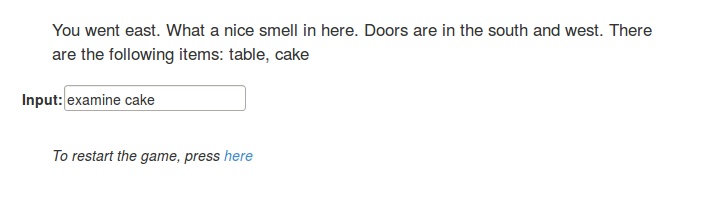
\includegraphics[scale=0.4]{screenshots/2015-03-25-104521_703x213_scrot.png}
    \caption{Aktion im zweiten Raum}
  \end{figure}
\end{frame}
% ---
\section{Struktur}
\subsection{Verwendete Techniken}
\begin{frame}
  \frametitle{Techniken}
  \begin{itemize}
    \item Yesod Framework
      \begin{itemize}
        \item Ausgabe der Ergebnisse bzw.\ Fehlermeldungen, z.B.\\ \emph{Invalid Input.}
        \item Aufbau der Startseite
        \item Formular zur Eingabe der Kommandos
      \end{itemize}
    \item Persistent
      \begin{itemize}
        \item Speichern des Spielerstatus
        \item Speichern der veränderten Items (z.B.\ Inventar)
        \item Bereitstellung der statischen Spielwelt
      \end{itemize}
    \item Monaden
      \begin{itemize}
        \item Handler-Monade
        \item Maybe-Monade
      \end{itemize}
  \end{itemize}
\end{frame}
% ---
\subsection{Aufbau des Codes}
\begin{frame}
  \frametitle{Handler und Templates}
  \begin{itemize}
    \item Home.hs mit homepage.hamlet
      \begin{itemize}
        \item Startseite
        \item Kurze Vorstellung des Spielprinzips
      \end{itemize}
    \item GameHome.hs
      \begin{itemize}
        \item Generierung einer zufälligen URL für den Spieler
        \item Weiterleitung zum Spiel
      \end{itemize}
    \item Game.hs mit game.hamlet und game.lucius
      \begin{itemize}
        \item Aufbau des Eingabefelds
        \item Verarbeitung der Eingabe
        \item Ausgabe des Ergebnisses
      \end{itemize}
  \end{itemize}
\end{frame}
% ---
\begin{frame}[fragile]
  \frametitle{Datenbank}
  \begin{itemize}
    \item Layout
      \begin{itemize}
        \item \verb|Area|
          {\tiny
            \begin{table}[!h]
              \begin{flushleft}
                \begin{tabular}{llllll}
                  area\_description & name & go\_north & go\_east & go\_south & go\_west \\ \hline
                  Text & Text Maybe & Int Maybe & Int Maybe & Int Maybe & Int Maybe
                \end{tabular}
              \end{flushleft}
            \end{table}
          }
        \item \verb|Item|
          {\tiny
            \begin{table}[!h]
              \begin{flushleft}
                \begin{tabular}{lllllll}
                  item\_description & name & use\_action & exact\_location & takeable & area\_id & UniqueItem \\ \hline
                  Text & Text & Text & Text Maybe & Bool & AreaId & name area\_id
                \end{tabular}
              \end{flushleft}
            \end{table}
          }
        \item \verb|Player_status|
          {\tiny
            \begin{table}[!h]
              \begin{flushleft}
                \begin{tabular}{llll}
                  area\_id & time & urlHash & UniqueHash \\ \hline
                  AreaId & UTCTime Maybe & Text & urlHash
                \end{tabular}
              \end{flushleft}
            \end{table}
          }
        \item \verb|Item_status|
          {\tiny
            \begin{table}[!h]
              \begin{flushleft}
                \begin{tabular}{lll}
                  player\_id & item\_id & status \\ \hline
                  Player\_statusId & ItemId & Text 
                \end{tabular}
              \end{flushleft}
            \end{table}
          }
        \item Nur \verb|Player_status| und \verb|Item_status| werden verändert.
      \end{itemize}
  \end{itemize}
\end{frame}
% ---
\begin{frame}[fragile]
  \frametitle{Datenbank}
  \begin{itemize}
    \item DbFunctions.hs
      \begin{itemize}
        \item Funktionen für den Datenbankzugriff, z.B.
          \begin{lstlisting}
getPlayer :: Text ->
  Handler (Maybe (Entity Player_status))
getPlayer urlHash = do
    runDB $ getBy $ UniqueHash urlHash
          \end{lstlisting}
      \end{itemize}
  \end{itemize}
\end{frame}
% ---
\begin{frame}[fragile]
  \frametitle{Actions.hs}
  \begin{itemize}
    \item Benutzt die Funktionen aus DbFunctions.hs
    \item z.B.\ Funktion zur Ausgabe der item\_description
    \begin{lstlisting}
examine :: Text -> Int64 -> Handler Text
examine obj areaId = do
    output <- lookAtItemByUnique obj areaId
    case output of
        Just (Entity _ itemVal) ->
            return $ itemItem_description itemVal
        Nothing ->
            return "No such item in this area."
    \end{lstlisting}
  \end{itemize}
\end{frame}
% ---
\begin{frame}[fragile]
  \frametitle{Parser.hs}
  \begin{itemize}
    \item Parsing des Inputs
      \begin{lstlisting}
parseInput :: Text -> Input
      \end{lstlisting}
    \item In eigenen Datentyp \verb|Input|
    \begin{lstlisting}
data Input = Input {
  act :: Maybe Action,
  obj :: Maybe Text
  } deriving (Show, Eq)
data Action = Go | Use | Open | Examine | PickUp |
  Inventory | LookAround | Eat deriving (Show, Eq)
    \end{lstlisting}
  \end{itemize}
\end{frame}
% ---
\section{Probleme}
\begin{frame}
  \frametitle{Probleme}
  \begin{itemize}
    \item Einarbeitung in das yesod-Framework und Persistent
    \item Generierung der zufälligen URL
    \item Verarbeitung von Eingaben in natürlicher Sprache
  \end{itemize}
\end{frame}
% ---
\section{Genutzte Bibliotheken und Codevorlagen}
\begin{frame}
  \frametitle{Bibliotheken und Codevorlagen}
  \begin{itemize}
    \item Yesod
    \item Persistent
    \item Code aus http://www.yesodweb.com/book/
  \end{itemize}
\end{frame}
% ---
\section{Verteilung der Aufgaben}
\begin{frame}
  \frametitle{Arbeitsteilung}
  \begin{itemize}
    \item Eva Braß
      \begin{itemize}
        \item DbFunctions.hs
        \item Design der Templates
        \item Aufbau der Spielwelt
      \end{itemize}
    \item Felix Reihl
      \begin{itemize}
        \item Actions.hs
        \item Parser.hs
      \end{itemize}
    \item Gemeinsam
      \begin{itemize}
        \item Struktur der Datenbank
        \item Handler
      \end{itemize}
  \end{itemize}
\end{frame}
% ---
\begin{frame}
  \centering Vielen Dank für die Aufmerksamkeit!
\end{frame}
% ---
\end{document}
